\ProvidesFile{seminar05.tex}

\section{Семинар 5}

\subsection{Задача 1}

Сколько существует способов переставить буквы в слове ОБОРОНОСПОСОБНОСТЬ
так, чтобы никакие две буквы О не стояли рядом?

Слово ОБОРОНОСПОСОБНОСТЬ содержит 7 букв <<О>> и 11 букв не <<О>>, а именно: 2 буквы Б, 2 буквы Н, 3 буквы С, остальные буквы по одному разу. Тогда ясно, что способов переставить <<не О>> $\frac{11!}{2! \cdot 2! \cdot 3!}$

Теперь давайте считать все буквы <<не О>> перегородками, а буквы <<О>> -- шарами. Тогда нужно в каждый промежуток между перегородками (а также до и после перегородок) поставить не более одного шара. Или другими словами, для каждого шара выбрать промежуток, куда мы его поставим, но при этом повторяться эти промежутки не могут.

Перегородок 11 штук, поэтому подходящих промежуток 12 (один слева от первой перегородки, 10 между перегородками, один справа от последней перегородки). Тогда для первого шара я могу выбрать один из 12 промежутков, для второго -- один из 11, $\ldots$, для седьмого -- один из шести. Но вообще говоря, я не различаю буквы О (шары) между собой, поэтому ещё нужно делить на 7! Получаем $C^7_{12}$.

Не забываем домножить на количество способов переставить буквы не О и получаем ответ.

\textbf{Ответ:} $C^7_{12} \cdot \frac{11!}{2! \cdot 2! \cdot 3!}$

\subsection{Задача 2}

Сколькими способами можно разделить 15 одинаковых монет между 7 нумизматами
так, чтобы каждому досталось хотя бы по монете?

Давайте всем ребятам сразу дадим по монетке, чтобы никого не обидеть. Тогда останется 8 монеток, которые нужно распределить между 7 ребятами.

Будем считать, что у нас 6 перегородок (на 1 меньше, чем число ребят), а 8 монеток -- шарами. Ну и все что нужно сделать -- это любыми способами расставить 8 шаров и 6 перегородок. Ясно, что число способов это сделать -- $C^6_{14}$

\textbf{Ответ:} $C^6_{14}$

\subsection{Задача 3}

Давайте сразу дадим всем числам по 5. Тогда останется раздать 75 между 5 числами. Поставим 4 перегородки и 75 шариков. Думаю, понятно, что всё, что идёт до первой перегородки -- идет в первое число, всё что идет между первой и второй перегородкой -- идёт во второе число ну и так далее.

79 мест и надо просто расставить 4 перегородки, на эти 79 мест. Итог: $C^4_{79}$

\textbf{Ответ:} $C^4_{79}$

\subsection{Задача 4}

Сколько существует способов представить число $n$ в виде суммы натуральных слагаемых, если способы, отличающиеся лишь порядком слагаемых, считаются различными?

Ясно, что слагаемых не более, чем $n$. Пусть слагаемых $k$ штук. Аналогично предыдущей задаче можно про это думать так: каждому из $k$ слагаемых мы раздали по единице. А оставшиеся $n - k$ можно распределять как угодно. Для этого нужно лишь расставить $n - k$ шаров и $k - 1$ перегородок. Ясно, что всего объектов $n$, а расстановка $k - 1$ перегородок однозначно задаёт всё. Поэтому число способов это сделать $C^{k-1}_{n}$.

Тогда всё что нужно сделать это взять сумму
\[
\sum_{k=1}^{n} C^{k-1}_{n} = \sum_{k=0}^{n-1} C^{k}_{n} = 2^{n-1}
\]
\textbf{Ответ:} $2^{n-1}$

\subsection{Задача 5}

Докажи тождество, не применяя формулу для количества сочетаний:
\[
C^k_n\cdot C^m_k = C^m_n \cdot C^{k-m}_{n-m}
\]

\begin{proof}
Слева написано следующее: сначала из $n$ человек выберем $k$ крутых ребят, а потом из $k$ крутых ребят выберем $m$ мега-крутых ребят.

Справа написано следующее: сначала из $n$ человек выберем $m$ мега-крутых ребят, а потом из оставшихся $n - m$ выберем $k- m$ просто крутых ребят. 

Ясно, что мы посчитали одно и то же двумя способами, что доказывает это тождество
\end{proof}

\subsection{Задача 6}
Докажи тождество, не применяя формулу для количества сочетаний:
\[
C^{k+1}_{n+1} = C^{k}_{n} + C^{k}_{n-1} + C^k_{n-2} + \ldots + C^k_k
\]
\begin{proof}
Заметим, что $C^{k+1}_{n+1} = C^{k}_{n} + C^{k+1}_{n}$. (Либо мы берем $n+1$ элемент и тогда среди оставшихся $n$ нужно выбрать ещё $k$, либо мы не берем $n + 1$ элемент и тогда среди оставшихся всё ещё нужно выбрать $k + 1$).

Аналогично можно расписать последнее слагаемое в этой сумме:
\[
C^{k+1}_{n+1} = C^{k}_{n} + C^{k+1}_{n} = C^{k}_{n} + C^{k}_{n-1} + C^{k+1}_{n-1}
\]
Продолжаем действовать аналогично и в итоге приходим к такой сумме:
\[
C^{k+1}_{n+1} = C^{k}_{n} + C^{k}_{n-1} + C^k_{n-2} + \ldots + C^k_k
\]
\end{proof}

\subsection{Задача 7}

\begin{enumerate}[label=\asbuk*)]
\item В столовой университета продается $n$ различных блюд. Илья каждый день ходит
в столовую и заказывает некоторый набор блюд, но со странным ограничением: ни в
какие два дня наборы блюд, которые он заказал, не должны повторяться. Какое максимальное количество дней Илья сможет так ходить в столовую и какое суммарное количество блюд он закажет за это время?
\item Из $n$ человек нужно выбрать команду и назначить в ней капитана. Команда может состоять и из одного человека, тогда он будет капитаном.) Сколько существует способов это сделать?
\item Используя пункты (а) и (б), докажи тождество:
\[
C^1_n + 2C^2_n + \ldots + nC^n_n = n \cdot 2^{n-1}
\]
\end{enumerate}

\subsubsection{Пункт А}
Ясно, что Илья сможет ходить в столовую $2^n$ дней, так как на наборе из $n$ элементов есть $2^n$ уникальных подмножеств (каждый элемент либо берем, либо не берем).

Какое число блюд Илья съест за это время? Фиксируем конкретное блюдо. Тогда на оставшихся $n - 1$ типах блюд он мог заказать всё что угодно (по 2 варианта для каждого типа блюда: берём в заказ, или не берём. Тогда для фиксированного типа блюда Илья съест их $2^{n-1}$.


Но так как различных типов блюд всего $n$, то всего блюд будет съедено $n \cdot 2^{n-1}$

\subsubsection{Пункт Б}
Можно взять в команду одного человека и из этого одного выбрать капитана. Можно взять в команду двух людей и из этих двоих выбрать одного капитаном. Можно взять в команду $k$ людей и из этих $k$ выбрать одного капитаном.

Ясно, что итоговое число способов будет равно:
\[
C^1_n + 2C^2_n + \ldots + nC^n_n
\]
\subsubsection{Пункт В}
\begin{proof}
Надо лишь понять, почему пункты а и б решают одну и ту же задачу. Ну, например, увидим задачу про блюда в задаче про капитанов. Давайте сначала выберем одного из $n$ людей капитаном, а затем из оставшихся $n -1$ людей каждого мы либо берём, либо не берём. Получается, что всего способов набрать команду таким образом ровно $n \cdot 2^{n-1}$. Это объясняет тождество 
\[
C^1_n + 2C^2_n + \ldots + nC^n_n = n \cdot 2^{n-1}
\]

В задаче про блюда это можно увидеть следующим образом: если Илья заказал набор из $k$ блюд, то он (удивительно) съест $k$ блюд. Способов выбрать $k$ блюд из $n$ всего $C^k_n$. Поэтому Илья съест следующее число блюд:
\[
C^1_n + 2C^2_n + \ldots + nC^n_n
\]
Ну а ранее мы уже показали, что эту же величину можно посчитать и как $n \cdot 2^{n-1}$
\end{proof}
 
\subsection{Задача 8}
В предыдущих задачах, а также в лонгриде мы доказывали нижеперечисленные тождества комбинаторным способом. Докажи эти тождества, используя бином Ньютона:

\begin{enumerate}[label=\asbuk*)]
\item $C_n^0 + C_n^2 + C_n^4 + \cdots = C_n^1 + C_n^3 + C_n^5 + \cdots$

\item $(C_n^0)^2 + (C_n^1)^2 + \cdots + (C_n^n)^2 = C_{2n}^n$

\item $C_n^1 + 2C_n^2 + 3C_n^3 + \cdots + nC_n^n = n \cdot 2^{n-1}$
\end{enumerate}

\subsubsection{Пункт А}

\begin{proof}
Нетрудно заметить, что $(1 - 1)^n = C^n_n\cdot 1^n \cdot (-1)^0 + C^{n-1}_n\cdot 1^{n-1} \cdot (-1)^1 + \ldots + C^{0}_n \cdot 1^0 \cdot (-1)^n$.

Слева написан ноль, поэтому давайте перенесем слагаемые, у которых цэшка написана с минусом влево (то есть у которых минус единица в четной степени). Тогда получим требуемое.
\end{proof}

\subsubsection{Пункт Б}
\begin{proof}
Нетрудно заметить, что $(1+x)^{n} \cdot (1+x)^{n} = (1 + x)^{2n}$

Раскроем по биному скобки слева, а именно посчитаем коэффициент при $x^n$:
\[(1+x)^{n} \cdot (1+x)^{n} = \sum_{k=0}^{n} = C^k_{n} \cdot C^{n-k}_{n} = \sum_{k=0}^{n} C^k_{n} \cdot C^{k}_{n} = \sum_{k=0}^{n} (C^k_{n})^2\]
А скобки справа раскрываются совсем просто, это просто $C^n_{2n}$. Это доказывает требуемое.
\end{proof}
\subsubsection{Пункт В}
\begin{proof}
\[
(x+1)^n = C^0_n + C^1_nx + \ldots + C^n_nx^n
\]
Продифференцируем по $x$:
\[
n \cdot (x + 1)^{n-1} = C^{1}_n + 2C^2_n\cdot x + \ldots + n C^n_n x^{n-1}
\]
Подставим $x = 1$:
\[
n \cdot 2^{n-1} = C^{1}_n + 2C^2_n\cdot + \ldots + n C^n_n
\]
\end{proof}
\subsection{Задача 9}
Докажи эти тождества, используя треугольник Паскаля:
\begin{enumerate}[label=\asbuk*)]
    \item $C_n^0 + C_n^2 + C_n^4 + \cdots = C_n^1 + C_n^3 + C_n^5 + \cdots$

    \item $(C_n^0)^2 + (C_n^1)^2 + \cdots + (C_n^n)^2 = C_{2n}^n$
\end{enumerate}
\subsubsection{Пункт А}
\begin{proof}
    Если $n$ четно, то достаточно воспользоваться симметрией треугольника Паскаля.

    Если же $n$ нечетно, то можно воспользоваться тем, что каждое число в треугольнике Паскаля получено из суммы двух чисел выше него и свести задачу к четному случаю, не хочу это подробно расписывать.
\end{proof}

\subsubsection{Пункт Б}
\begin{proof}
Интерпретация правой части такая: оказывается, что $C^n_{2n}$ - количество путей из верха треугольника Паскаля до $C^n_{2n}$ (и вообще число путей до $C^k_{n}$ в треугольнике Паскаля равно $C^k_{n}$, так как по сути на каждом <<шаге>> из вершины треугольника вы можете пойти либо вправо, либо влево, следовательно, достаточно выбрать $k$ раз, когда вы пойдете вправо)

А что написано в левой части? Смотрите: чтобы дойти до точки $C^n_{2n}$ нужно сделать $n$ шагов влево и $n$ шагов вправо.

Тогда просто нужно выбрать стрелки влево, оставшиеся - будут стрелки вправо.

Но $n$ стрелок влево можно выбрать так: из первых $n$ выбираем 0 стрелок влево, из последних $n$ выбираем $n$ стрелок влево. Либо из первых $n$ стрелок выбираем 1 стрелку влево, из последних $n$ выбираем $n-1$ стрелку влево. Ну и так далее. Итог: $C^0_n C^n_n + C^1_n C^{n-1}_n + \ldots C^n_n C^0_n$.

Вот и получается, что мы посчитали одно и то же двумя способами.
\end{proof}

\subsection{Задача 10}
Сколькими способами можно разрезать правильный $n$-угольник на треугольники, проводя непересекающиеся диагонали?

\begin{claim*}
Для правильного $n$-угольника количество его триангуляций равно $c_{n-2}$ ($c_k$ - кол-во правильных скобочных последовательный из $2k$ скобок).
\end{claim*} 

\begin{proof}
    Давайте просто покажем, что между триангуляциями и правильными скобочными последовательностями (ПСП) есть биекция. Это объяснит наше утверждение. 

    \begin{figure}[H]
        \centering
        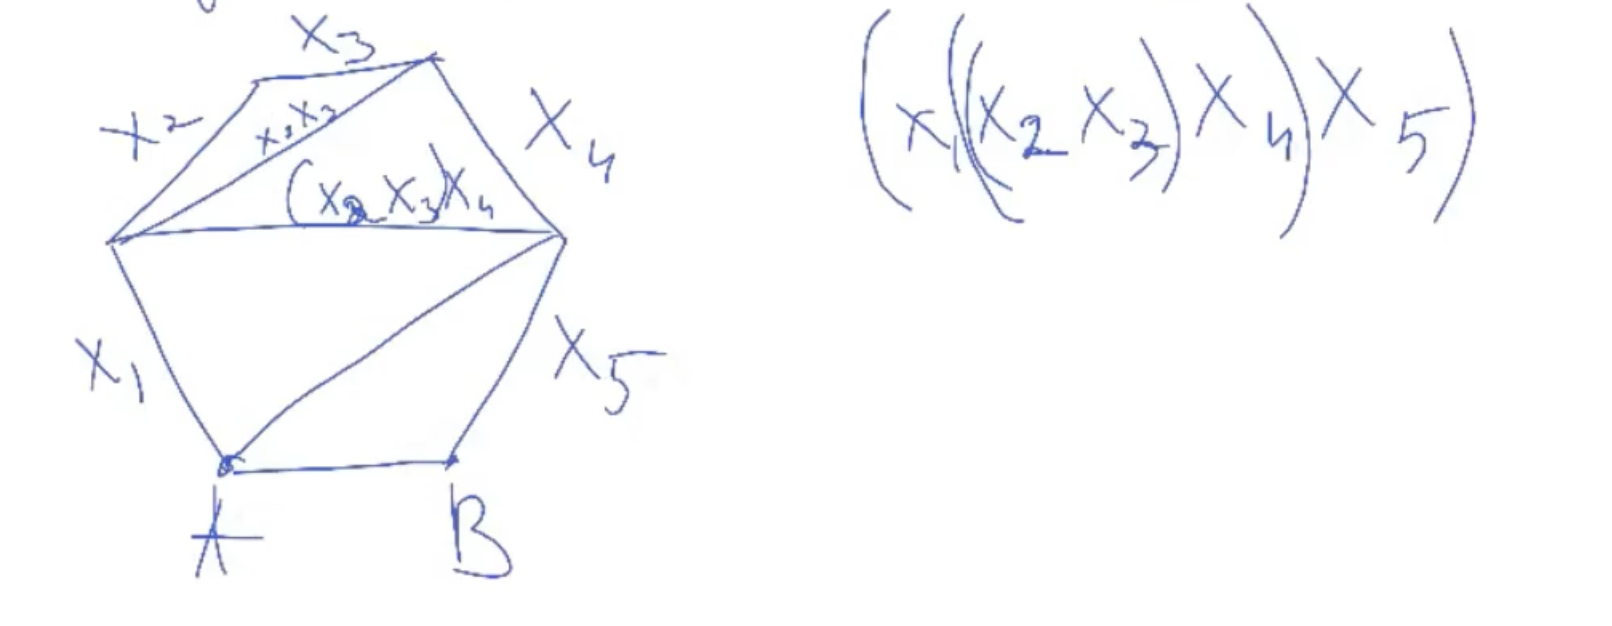
\includegraphics[width=1\linewidth]{Figures/sem05_task10.png}
    \end{figure}

    Думаю, по этой картинке понятно, как устроена биекция и как получать картинку из ПСП и наоборот. Не хочется подробно расписывать =)
\end{proof}

\subsection{Задача 11}
На окружности отмечено $2n$ различных точек. Сколькими способами можно провести
$n$ попарно непересекающихся хорд, соединяющих эти точки, так, чтобы каждая точка
была концом ровно одной из проведенных хорд?

\begin{claim*} 
Для правильного $2n$ различных точек число искомых способов равно $c_n$
\end{claim*}

\begin{proof}
Давайте просто покажем, что между выбором хорд и правильными скобочными последовательностями (ПСП) есть биекция.

\begin{figure}[H]
    \centering
    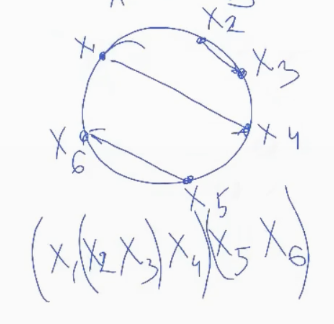
\includegraphics[width=0.5\linewidth]{Figures/sem05_task11.png}
\end{figure}
Опять же не хочу ничего подробно распмсывать, картинка многое объясняет, ну, разве что стоит немного аккуратно поговорить про то, что хорды не пересекаются, но я не хочу этим заниматься. 
\end{proof}